\documentclass[paper=a4,10pt]{scrartcl}

\usepackage[utf8x]{inputenc}
\usepackage[ngerman]{babel}
\usepackage[T1]{fontenc}

\usepackage{graphicx}
\usepackage{float}
\usepackage{subcaption}

\usepackage{fancyref}

\usepackage[numbers,square,sort]{natbib} %praktikumsquellenvorgabe
\usepackage{amsmath}
\usepackage{amssymb}

\usepackage{url}
\usepackage{hyperref}

\usepackage{bm}
\usepackage{siunitx}		% um SI-Einheiten richtig zu schreiben

\usepackage[a4paper, includehead, includefoot]{geometry}
\geometry{left=2cm, right=2cm, top=2cm, bottom=2cm}

\begin{document}

\title{NBTI-Theorie}
%\author{Author's Name}
\section{Begriffe}
\paragraph{$N_A$, $N_D$}: Die Dichten der für die Dotierung verwendeten Akzeptoren, bzw. Donatoren
\paragraph{$N_V$, $N_C$}: die effektiven Zustandsdichten, welche über Approximation der Anzahl der Zustände zB im Leiungsband erhalten werden (siehe Section \ref{seq:ladungskonz} und \ref{sec:effZD}). $N_V$ .. Valenzband, $N_C$ .. conduction Band.
\paragraph{$n_e$ bzw $n_n$ und $n_h$ bzw $n_p$} Ladungsträgerkonzentrationen/Dichte in den jeweiligen Bändern

\paragraph{intrinsischer Halbleiter} Ein reiner Halbleiter mit wenig bis keiner Dotierung. 

\paragraph{Flatband voltage} Wenn im Oxid oder an der Oxid-Halbleiter Schnittstelle keine Ladung vorhanden ist entspricht die Flatbandvoltage einfach der Austrittsarbeitesdifferenz zwischen Gatemetall und Halbleiter.

\paragraph{n-Typ, n-Kanal, NMOS, n-leitend} Diese Begriffe stehen alle für einen Transistor bei welchem Elektronen im Kanal die Ladung transportieren. Grundlage dafür ist ein p-dotiertes Substrat. Analog gilt das selbe für p-Typ, etc. 

\paragraph{Donor-like trap} Donors geben ein Elektron ans Leitungsband ab, während Akzeptoren ein Elektron aus dem Valenzband akzeptieren.

\section{Grundlagen}

\subsection{Work function}
Ist das selbe wie die Austrittsarbeit. Das ist die Energie, die mindestens aufgewandt werden muss, um ein Elektron aus einem ungeladenen Festkörper zu lösen.
In einem Halbleiter ist die work function abhängig von der Dotierung an der Oberfläche und da die Ladungsträgerkonzentration durch ein elektrisches Feld an der Oberfläche verändert werden kann, ist sie auch davon abhängig.

\subsection{Basic Band Theory}
Fangen an mit freiem Elektronengasmodel mit nur einem Elektron in einem Potentialtopf der breite $L$, welcher den Kristall darstellen soll. In diesem Fall kann anscheinend die Energie des Elektrons nur vollständig in kinetischer Form vorliegen. Jetzt wird die zeitunabhängige Schrödingergleichung  mit Potential gleich 0 und periodischen Randbedingungen gelöst zu:
\begin{align}
\psi = \left( \frac{1}{L}	\right)^{3/2} \cdot e^{i  \bm k \bm r}
\end{align}
mit $k_x = \pm n_x \cdot 2\pi / L$ mit der Quantenzahl $n_x=0,1,2,\dots$ und genauso für die anderen beiden Komponenten von $\bm k$.\\
Für die Geschwindigkeit des Elektrons erhält man 
\begin{align}
\bm v = \frac{\bm p}{m_e} = \frac{\hbar \cdot \bm k}{m_e}.
\end{align}
Da die total Energy hier identisch mit $E_{\text{kin}}$ ist, gilt
\begin{align}
E = \frac{m_e v^2}{2} = \frac{\hbar^2 \bm k^2}{2m_e} = \frac{\hbar^2}{2m_e} \left( \frac{2\pi}{L} \right)^2 (n_x^2 +n_y^2 + n_z^2)
\end{align}
Das ist eine Dispersionsrelation, weil $E$ durch $\bm k$ ausgedrückt wird.
Diese ganze Herleitung ist dazu da gewesen, um zu zeigen, dass die Energiewerte nur diskret sein können. Dieses Ergebnis ist auch dann noch gültig, wenn man mit den korrekten Potentialen rechnet und mehrere Elektronen betrachtet. Der Zusammenhang zwischen $E$ und $\bm k$ wird dann jedoch deutlich komplexer.\\
Jetzt wo die Energielevel bekannt sind, kann man zählen, wie viele Energielevel es in einem Energieintervall $\Delta E$ bei der Energie $E$ gibt. Das macht man im $k$-Raum, im phase space.

Im phase space ist eine Fläche konstanter Ebene eine Sphäre, da alle Punkte, deren $\bm k$ die selbe Länge haben auch den selben Energiewert besitzen.
Jeder Zustand (jede Lsg. der Schrödingergleichung) mit einem bestimmten $\bm k$ nimmt ein Volumen ein (kleine Würfel).
Die Anzahl of cubes die in die Sphäre zur Energie $E$ passen ist die Zahl aller Energiezustände bis zu $E$.

Jetzt wollen wir die density of states $D(E)$ ermitteln.

Ein einzelner Zustand nimmt im $\bm k$-Raum ein Volumen von $(2\pi)^3/V$ mit $V=L_xL_yL_z$ und mit dem Faktor 2 für die Spinentartung hat man einen Zustand pro diesem Volumen -> $Z(\bm k) = 2 \cdot V/(2\pi)^3$. 

Die Zustandsdichte im Energieraum erhält man mit der Dispersionsrelation von oben und der Beziehung
\begin{align}
Z(\bm k) d^3k = D(E)dE.
\end{align} 
\textit{Wo kommt das her?}

Die Herleitung im Marx ist für mich immer durch irgendwelche Approximationen nicht konkret genug. Jedoch kommt dabei das überall stehende Ergebnis mit $D(E) \sim \sqrt{E}$ raus.

\section{Fermi-Verteilung}
Sie gibt die Wahrscheinlichkeit dafür, dass ein Platz bei der Energie $E$ und Temperatur $T$ in einem System von Fermionen, das durch die Fermienergie $E_F$ charakterisiert ist, besetzt ist.
Ein System , bei dem die Besetzung der verfügbaren Plätze dieser Verteilung folgt, ist automatisch im thermodynamischen Gleichgewicht, d.h. es hat die kleinstmögliche freie Energie $G = E-TS$.
\begin{align}
f(E;E_F, T) = \frac{1}{e^{\frac{E-E_F}{k_BT}}+1}
\end{align}
Die Fermienergie ist die Energie bei der $f(E_F; E_F, T) = 1/2$ gilt. Für sie gilt, dass sie wenn man T gegen Null gehen lässt angibt welche Energie der letzte noch besetzt Platz hat.
Die Fermienergie ist bzgl $E_F$ punktsymmetrisch und man kann sie für $E-E_F > 2k_BT$ durch die Boltzmannnäherung ersetzen:
\begin{align}
f(E,T) \approx e^{-\frac{E-E_F}{k_BT}}
\end{align}

\section{Ladungsträgerkonzentration etc.}
\label{seq:ladungskonz}
Die Frage nach der Anzahl an Zuständen im Leitungsband bei geg. Temperatur $T$ wird wie folgt beantwortet: Die Dichte der Elektronen bei Energie $E$ ist gleich die Zahl der vorhandenen Plätze (Zustandsdichte $D(E)$) mal die Wahrscheinlichkeit der Besetzung ($f(E)$) und das dann über alle Energien aufsummiert (integriert).

\textit{Also wie viele Zustände gibt es mal die Wahrscheinlichkeit diese auch zu besetzen?}
Mit Boltzmann Näherung und Abschätzung durch $N_{\text{eff}}$ wird die Dichte der Elektronen im Leitungsband dann noch abgeschätzt:
\begin{align}
n_e &= \int^{\infty}_{E_L} D(E) f(E; E_F, T) dE \label{eq:ne} \\ 
&\approx N^C_{\text{eff}} \;  e^{-\frac{E_L-E_F}{k_B T}} \label{eq:ne2}
\end{align}
Die untere Gleichung definiert $N_{\text{eff}}$.

Jetzt wollen wir die Dichte der Löcher berechnen. Die Dichte der Löcher zur Energie $E$ ist gleich der Zahl der vorhandenen Plätze ($D(E)$) mal die Wahrscheinlichkeit der Nichtbesetzung ($1-f(E)$):
\begin{align}
n_h &= \int_{-\infty}^{E_V} D(E) [1-f(E; E_F, T)] dE \label{eq:nh} \\
&\approx N^V_{\text{eff}} \;  e^{-\frac{E_F-E_V}{k_B T}} \label{eq:nh2}
\end{align}
\subsection{Massenwirkungsgesetz}
Für den perfekten (intrinsischen) Halbleiterkristall stammen alle Elektronen im Leitungsband aus dem Valenzband:
\begin{align}
n_e = n_h =: n_i
\end{align}

Das Massenwirkungsgesetz lässt sich wie folgt über \ref{eq:ne} und \ref{eq:nh} berechnen). Durch Gleichsetzen von $n_e$ und $n_h$ im intrinsischen Fall erhält man:
\begin{align}
n_i = N_{\text{eff}} \; e^{-\frac{E_L-E_V}{2k_BT}} = N_{\text{eff}} \; e^{-\frac{E_G}{2k_BT}}
\label{eq:intri_gleich}
\end{align}
(Dabei geht mit ein, dass in diesem Fall wohl die effektiven Zustandsdichten gleich sind, weil sonst könnte man die nicht wegkürzen um den einfachen Ausdruck $E_F = \frac{E_L + E_V}{2}$ für die Fermienergie zu erhalten den man dann einsetzen kann.)
Wenn man jetzt $n_e$ und $n_h$ miteinander multiplizert erhält man:
\begin{align}
n_e \cdot n_h = N^2_{\text{eff}} \; e^{2\frac{-E_L + E_F - E_F + E_V}{2k_BT}} = n_i^2
\end{align}
Da aber für die letzte Rechnung gar nicht vorgegeben war, dass es sich um einen intrinsischen HL handelt, gilt allgemein das Massenwirklungsgesetz:
\begin{align}
n_e \cdot n_h = n_i^2 \label{mwg}
\end{align}

Die Energielücke und die intrinsische Ladungsträgerdichte stellen im Grunde den selben Materialparameter dar:
\begin{align}
n_i = N_{\text{eff}} e^{- \frac{E_L-E_F}{k_BT}}
\end{align}
\section{effektive Zustandsdichte}
\label{sec:effZD}
Sie ist diejenige Zustandsdichte (Zahl der Zustände pro Volumen), die von Elektronen im Leitungsband, bzw Löchern im Valenzband besetzt werden können und bei der statt der Masse des Elektrons die effektive Masse für das jeweilige Band eingesetzt werden muss.
Für das Leitungsband zB:
\begin{align}
N_C = 2 \cdot \left( \frac{2 \pi m^* k_B T}{h^2} \right)^{\frac{3}{2}} \cdot M_C
\end{align}
wobei $M_C$ die Anzahl der Energieminima des Bandes entspricht. Die effektive Zustandsdichte wird benötigt, um die Zahl der Ladungsträger im Leitungsband zu berechnen (ich glaube siehe \ref{seq:ladungskonz}).

\section{Ladungsträgerkonzentration}
\label{sec:carrier_concentration}
Ist die Anzahl der zum elektrischen Strom beitragenden Ladungsträger pro Volumen (also eine Art Dichte).

Uni-Kiel Seite:\\
Die Konzentrationen der Elektronen/Löcher ergeben sich ja über das Produkt der Zustandsdichte mit der Fermi-Verteilung und anschließende Integration darüber. Die entscheidende Größe, die den Wert des Integrals massiv beeinflussen kann ist der 'Zipfel' der fermi-Verteilung, der oberhalb bzw unterhalb der Bandlücke herausragt.
\textit{Das wird damit begründet, dass man die Zustandsdichte durch die 'wirkliche Zustandsdichte' einigermaßen ersetzen kann und das eine Art Konstante ist, wobei ich nicht weiß, was mit 'wirkliche Zustandsdichte' gemeint ist.}

\section{degenerate Halbleiter}
In nicht degenerate (entartet?) Halbleitern ist laut Sze die Dopingkonzentration kleiner als $N_C$ und die Ferminiveaus liegen mehr als einig Vielfache von $kT$ unter $E_C$. Die Approximationen (\ref{eq:ne2}) und (\ref{eq:nh2}) gelten wohl anscheinend für nicht degenerate Halbleiter. \\

Für degenerate Level wo die n- oder p-Konzentrationen nah an effektiven Zustandsdichten liegen oder sogar größer sind muss man statt der Boltzmannnäherung den Wert des Fermi-Dirac Integrals nutzen. \\

Ein intrinsischer Halbleiter ist per Definition non degenerate
\section{Dotierung}
Wenn man ein Phosphoratom in einen Siliziumkristall einbringt bleibt nach der Bindung mit vier Nachbarsiliziumatomen ein Elektron übrig, welches nur leicht an das Phosphoratom gebunden ist. Eine kleine Energie (ca. \SI{50}{\milli\volt}) reichen aus, um es zu lösen und damit ins Leitungsband zu heben. Die solche Dotierung, welche Elektronen hinzufügt nennt man n-Dotierung. Im Bändermodell liegen die Phosphoratomzustände also etwas unter dem Leitungsband.\\
Wenn man ein ein Boratom (Akzeptor) einbringt, bleibt nach der Bindung ein Loch, welches mit wenig Energie von einem Elektron im nahegelegenen Valenzband besetzt werden kann, was dann dafür sorgt, dass sich nun ein Loch im Valenzband befindet.\\\\
Dotierung beeinflusst die Lage der Fermienergie.

Das Massenwirkungsgesetz (\ref{mwg}) gilt anscheinend auch erstmal für dotierte Halbleiter aber nur bis degeneracy, da für degenerate HL $np < n_i^2$ gilt. 
\textit{Aber ich weiß jetzt nicht wo der Unterschied oder Übergang ist.}

\section{Fermi-Energie}
Sie ist über den Energiewert definiert, bei welchem die Fermi-Verteilung gleich 1/2 ist.

\subsection{intrinsischer Halbleiter}
Im intrinsische HL herrscht Ladungsneutralität, dh. zu jedem Elektron gibt es auch ein Loch. Die Dichte der Elektronen im Leitungband ist also identisch zur Dichte im Valenzband.

\textit{Ausdrücke wie 'im Valenzband' beziehen sich nicht auf Orte, sondern auf Energien}

Da in Section \ref{sec:carrier_concentration} beschrieben wird, dass die Ladungsträgerkonzentrationen stark von den Fermi-Verteilungszipfeln abhängen und im intrinsischen Fall ja gleich sind, müssen die Zipfel sowohl im Valenz, als auch im Leitungsband gleichweit aus der Lücke herausragen und da die Verteilung symmetrisch ist, muss die Fermienergie ziemlich genau in der Mitte der Bandlücke liegen.
Wenn ich die Ladungsträgerdichten aus (\ref{eq:intri_gleich}) gleichsetze, dabei die effektiven Zustandsdichten unterscheide und nach $E_F$ auflöse, erhalte ich für die Fermienergie im intrinschen Fall:
\begin{align}
E_F = E_i \approx \frac{E_V + E_C}{2} + \frac{kT}{2} \ln \left( \frac{N_V}{N_C} \right)
\end{align} 

und damit kann man $n_i$ auch nochmal etwas genauer aufschreiben als:
\begin{align}
n_i = N_C e^{-\frac{E_C-E_i}{kT}} = N_V e^{-\frac{E_i - E_V}{kT}} = \sqrt{N_V N_C} \exp \left( - \frac{E_g}{2kT} \right)
\end{align}

\subsection{dotierter Halbleiter}
Sagen wir, wir haben einen mit Donatoren dotierten n-dotierten Halbleiter. Für geringe Temperaturen schaffen es mehr Elektronen von den Donatorniveaus, die etwas höhere Energien haben als die Valenzbandkante, ins Leitungsband. Bezeichnen wir mit $n_L(T)$ die Zahl (oder Volumendichte (gilt wohl für beides)) und mit $N^+_D(T)$ die Zahl der nicht mehr besetzten Zustände bei den Donatoratomen.
Wir schreiben nun $n_L$ entsprechend (\ref{eq:ne2}) und sagen außerdem allgemein via der Fermi-Verteilung (die gibt ja allg. die Wahrscheinlichkeiten für Besetzung bei geg. Energie für Fermionen an), dass die Zahl (Volumen) der noch von Elektronen besetzten Donatorzustände $N_D^0(T)$ der Zahl der Zustände mal die Besetzungswahrscheinlichkeit entspricht. Dadurch ergibt sich für $N^+_D$:
\begin{align}
N^+_D = N_D - N^0_D = N_D \cdot \left( 1 - f(E_D; E_F, T)\right) 
\end{align}

Wenn ich so $n_L(T)$ und $N^+_D(T)$ gleichsetze, weil ich das ja für kleiner Temperaturen machen kann, kann man zeigen, dass die Fermienergie zwischen $E_L$ und $E_D$ liegt.

Schaut man sich jetzt nochmal $n_V$, die Ladungsträgerdichte von Löchern im Valenzband an, die sich über (\ref{eq:nh2}) ergibt, hat man nun, da $E_F$ größer geworden ist als im intrinsischen Fall und es wird klar, dass man durch dir n-Dotierung nun mehr Elektronen im Leitungsband als Löcher im Valenzband hat.

Das war alles bisher nur für kleine Temperaturen bei welchen die Zahl der Elektronen die es aus dem Valenzband ins Leitungsband schaffen vernachlässigt werden kann. \\\\
Jetzt nehmen wir eine so hohe $T$ an, dass es garantiert mehr Elektronen aus dem Valenzband schaffen, als es Donatoren gibt. Damit ist der Unterschied zum intrinsischen Verhalten kaum mehr zu unterscheiden und die Fermienergie ist wie im intrinsischen Fall wieder in der Bandmitte.\\
Bei hohen Temperaturen liegt sie also in der Mitte und bei niedrigen zwischen $E_L$ und $E_D$. Bei mittleren Temperaturen kann sie also nur irgendwo dazwischen liegen und man erwartet, dass sie für höhere Donatorkonzentrationen später in Richtung Mitte wandert, da es mehr Elektronen aus dem Valenzband benötigt, um die Zahl an Donatorelektronen zu überwiegen.

\begin{figure}[H]
\centering
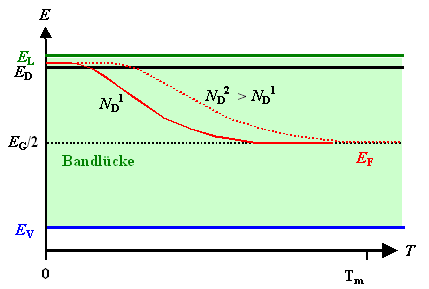
\includegraphics[scale=0.7]{../bilder/fermi_temperatur.png}
\caption{Lage der Fermienergie bei n-dotierten Halbleitern in Abhängigkeit der Temperatur.}
\label{fig:fermi_n}
\end{figure}

Für p-dotierte Halbleiter sieht das folgendermaßen aus:

\begin{figure}[H]
\centering
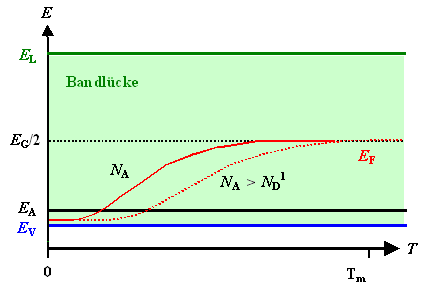
\includegraphics[scale=0.7]{../bilder/fermi_temperatur2.png}
\caption{Lage der Fermienergie bei p-dotierten Halbleitern in Abhängigkeit der Temperatur.}
\label{fig:fermi_p}
\end{figure}

Die Dotierzustände liegen nah am Valenzband und so ist es bei geringer Temperatur möglich, dass Elektronen vom Valenzband in die Akzeptorzustände springen und es mehr Löcher im Valenzband gibt als Elektronen im Leitungsband. Das Ferminiveau liegt zwischen $E_V$ und $E_A$ und es gibt mehr Löcher im Valenzband als Elektronen im Leitungsband.

\subsection{bei Metallen}
Bei Metallen ist die Fermienergie die Austrittsarbeit.

\section{pn-Übergang}
Wenn man zwei unterschiedlich dotierte Halbleiter verbindet ist das Gesamtkonstrukt zwar immernoch elektrisch neutral, es gibt aber einen Konzentrationsgradienten von Ladungsträgern. Die Majos wandern durch Diffusion ins andere Gebiet, in dem die entsprechende Konzentration geringer ist. Auf beiden Seiten gibt es nun Rekombination und auf beiden Seiten fehlen nun Ladungsträger in den vorher ungeladenen Materialien. Die zu den fehlenden beweglichen Ladungsträgern gehörenden Dotieratome verursachen nun ein elektrisches Feld aufgrund ihrer nicht mehr kompensierten Raumladungen. Die dadurch resultierende Driftbewegung ist der Diffusionsbewegung entgegenwirkend und es kommt zu einem Gleichgewicht. Das entstandene el. Feld drückt die verbleibenden freien Ladungsträger zurück und es entsteht beiderseits der Grenze eine Verarmungszone ohne freie Ladungsträger in der nur noch die ortsfesten Raumladungen verbleiben (deshalb auch Raumladungszone).

Die Ausdehnung der Verarmungszone ist abhängig von der Dotierung der Zone und der intrinsichen Ladungsträgerdichte des Materials. Bei gleich hoher Dotierungsdichte von n- und p-Gebiet ist die Zone symmetrisch. Bei ungleichen Dotierungsdichten breitet sich die RLZ weiter in das weniger stark dotierte Gebiet aus.

\textit{Das erkläre ich mir über die stärkere Diffusion in das weniger stark dotierte Gebiet. Wenn im linken Gebiet eine höhere n-Dotierung als p-Dot. rechts vorliegt, ist die Bewegung aufgrund des Drifts stärker von links nach rechts, weil der Gradient größer ist. Dadurch findet auch mehr Rekombination rechts statt, würde ich sagen.}

Nach dem Kontakt muss es ein gemeinsames Equilibrium geben mit const. Fermienergie. Weit weg vom Übergang haben die HL ihre intrinsischen Eigenschaften

Betrachtet man das Bändermodell, so haben sich die Fermi-Niveaus durch den Diffusionsprozess angeglichen und es zeigt sich eine Krümmung der Energiebänder im Bereich des p-n-Übergangs.




\section{Erklärungen}
\subsection{Bias}
\textit{Bisher habe ich das so verstanden, dass das einfach die Spannung ist, die zwischen Source und Gate angelegt ist.} \\

\noindent
In einem Paper über NBTI (Statistical Model for MOSFET Bias TemperatureInstability Component Due to Charge Trapping von G. Wirth) steht, dass bei konst. Bias nur states (traps) nahe des Fermilevels eine starke Aktivität aufweisen, also ihren Zustand zwischen besetzt und leer wechseln. Das kann man als steady state condition interpretieren -> occupation probability of a trap is time independent -> Anzahl an Traps die als besetzt erwartet werden ist konstant. Falls der bias point sich abrupt ändert, ändert sich auch die Besetzungswahrscheinlichkeit abrupt.
\textit{Intuitiv kann ich das nicht einordnen.}

\subsection{threshold voltage}
Das ist die minimale Gate-Source Spannung, die angelegt sein muss, damit eine leitende Brücke zwischen source und drain entsteht.


\end{document}